\documentclass[IA.tex]{subfiles}

\begin{document}
\newcommand{\graphFunc}{\draw[darkgray, smooth, thick, samples=100, domain=2:8] plot(\x,{cos(\x r)+1}) node[darkgray, align=left, right, yshift=0.5cm, xshift=-3.9cm] {\scriptsize \(f(x)\)};}
\newcommand{\trapezoid}{
    \draw [gray, thin] (BL) -- (BR);
    \draw [gray, thin] (BR) -- (TR);
    \draw [gray, thin] (TR) -- (TL);
    \draw [gray, thin] (TL) -- (BL);
    \fill [pattern=north west lines, pattern color=gray] (BL) to (TL) to (TR) to (BR);
}
\begin{figure}[ht]
    \centering
    \resizebox{.6\textwidth}{!}{
        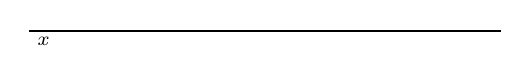
\begin{tikzpicture}[extended line/.style={shorten >=-#1,shorten <=-#1}]
            \coordinate (BL) at (2, 0);
            \coordinate (BR) at (4, 0);
            \coordinate (TL) at (2, 0.584);
            \coordinate (TR) at (4, 0.346);
            \trapezoid

            \coordinate (BL) at (4, 0);
            \coordinate (BR) at (6, 0);
            \coordinate (TL) at (4, 0.346);
            \coordinate (TR) at (6, 1.960);
            \trapezoid

            \coordinate (BL) at (6, 0);
            \coordinate (BR) at (8, 0);
            \coordinate (TL) at (6, 1.960);
            \coordinate (TR) at (8, 0.854);
            \trapezoid

            \draw[black, thick] (2, -0.02) -- (8, -0.02) node[black, align=center, left, yshift=-0.13cm, xshift=-5.6cm] {\scriptsize \(x\)};
            \graphFunc
        \end{tikzpicture}
    }
    \vspace{-.9cm}
    \caption{Trapezoid Rule}
    \label{fig:trap_rule}
\end{figure}
\end{document}
